\section*{Overview}
In the last chapter of this thesis, we propose VarFA, a variational inference factor analysis framework that extends existing factor analysis models for educational data mining to efficiently output uncertainty estimation in the model's estimated factors. Such uncertainty information is useful, for example, for an adaptive testing scenario, where additional tests can be administered if the model is not quite certain about a students' skill level estimation. Traditional Bayesian inference methods that produce such uncertainty information are computationally expensive and do not scale to large data sets. VarFA utilizes variational inference which makes it possible to efficiently perform Bayesian inference even on very large data sets. We use the sparse factor analysis model as a case study and demonstrate the efficacy of VarFA on both synthetic and real data sets. VarFA is also very general and can be applied to a wide array of factor analysis models. Code and instructions to reproduce results in this chapter are available from~{\color{blue}{\url{https://tinyurl.com/tvm4332}}}.
\section{Introduction}
\label{sec:intro}
%
A core task for many practical educational systems is \textit{student
    modeling}, i.e., estimating students' mastery level on a set of skills or
knowledge components (KC)~\cite{vanlehn1988student, chrysafiadi2013student}.
Such estimates allow in-depth understanding of students' learning status and
form the foundation for automatic, intelligent learning interventions. For
example, intelligent tutoring systems (ITSs)~\cite{shute1994intelligent,
    pls1,anderson1995cognitive,nye2014autotutor,heffernan2014assistments,rafferty2015inferring}
rely on knowing the students' skill levels in order to effectively recommend
individualized learning curriculum and improve students' learning outcomes. In
the big data era, student modeling is usually formulated as an educational data
mining (EDM)
problem~\cite{romero2010educational,baker2009state,merceron2005educational}
where an underlying machine learning (ML) model estimates students' skill
mastery levels from students' learning records, i.e., their answers to
assessment questions.

\sloppy
Many student modeling methods have been proposed in prior literature. A fruitful line of research for student modeling follows the \textit{factor analysis (FA)} approach.
FA models usually assume that an unknown, potentially multi-dimensional student parameter, in which each dimension is associated with a certain skill, explains how a student answers questions and is to be estimated. Popular and successful FA models include item response theory (IRT)~\cite{irt}, multi-dimensional IRT~\cite{mirt}, learning factor analysis (LFA)~\cite{LFA}, performance factor analysis (PFA)~\cite{PFA}, DASH (short for {d}ifficulty, {a}bility, and {s}tudent {h}istory)~\cite{lindsey2014improving,mozer2016predicting}, DAS3H (short for {d}ifficulty, {a}bility, {s}kill and {s}tudent {s}kill {h}istory)~\cite{das3h}, knowledge tracing machines (KTM)~\cite{vie2019knowledge}, and so on.
% 
Recently, more complex student models based on deep neural networks (DNN) have
also been proposed~\cite{DKT,zhang2017dynamic,minn2018deep}. Nevertheless,
thanks to their simplicity, effectiveness and robustness, FA models remain
widely adopted and investigated for practical EDM tasks. Moreover, there is
evidence that simple FA models could even outperform DNN models for student
modeling in terms of predicting students' answers~\cite{irt-best}. Because of
FA models' competitive performance and its elegant mathematical form, we focus
on FA-based student models in this chapter.

Most of the aforementioned FA models compute a single point estimate of skill
levels for each student. Often, however, it is not enough to obtain mere point
estimates of students' skill levels; knowing the model's uncertainty in its
estimation is crucial because it potentially helps improve the model's
performance and improve both students' and instructors' experience with
educational systems.
% 
For example, in ITS, an underlying model can use the uncertainty information in
its estimation of students' skill level to automatically decide that its
recommendations based on highly uncertain estimations are unreliable and
instead notify a human instructor to evaluate the students' performance. This
enables collaboration between ITS and instructors to create a more effective
learning environment.
%
In adaptive testing systems~\cite{chang2009nonlinear,yan2016computerized},
knowing the uncertainty in model's estimation could help the model
intelligently pick the next test items to most effectively reduce its
uncertainty about estimated students' skill levels. This will help to
potentially reduce the number of items needed to have a confident, accurate
estimation of the students' skill mastery level, saving time for both students
to take the test and instructors to have a good assessment of the student's
skills.

All the above applications require the model to ``know what it does not know,''
i.e., to quantify the uncertainty of its estimation. Achieving this does not
necessary changes the model. rather, we need a different inference algorithm
for inferring not only a point estimate of student's skill level from observed
data (i.e., students' answer records to questions) but also uncertainty in the
estimations.

Fortunately, there exist methods that both compute point estimates of students'
skill levels and quantifies the uncertainty of those estimates. These methods
usually follow the Bayesian inference paradigm, where each student's unknown
skill levels are treated as random variables drawn from a \textit{posterior
    distribution}. Thus, one can use the \textit{credible interval} to quantify the
model's uncertainty on the student's estimated skill level. A classical method
for Bayesian inference is Monte Carlo Markov Chain (MCMC)
sampling~\cite{gelman2013bayesian} which has been widely used in many other
disciplines~\cite{gilks1995markov} other than EDM. In the context of student
modeling with FA models, existing works such as
~\cite{lan14a,fox2010bayesian,pardos2010using,merkle2011comparison} have
applied MCMC methods to obtain credible intervals.

Unfortunately, classic Bayesian inference methods suffer from extensive
computational complexity. For example, each computation step in MCMC involves a
time-consuming evaluation of the posterior distribution. Making matters worse,
MCMC typically takes many more steps to converge than non-Bayesian inference
methods. As a concrete illustration, in~\cite{lan14a}, the Bayesian inference
method (10 minutes) is about 100 times slower than the other non-Bayesian
inference method based on stochastic gradient descent (6 seconds). The high
computational cost prevents Bayesian inference methods from mass-deployment in
large-scale, real-time educational systems where timely feedback is critical
for learning~\cite{driscoll1994psychology} and tens of thousands of data points
need to be processed in seconds or less instead of minutes or hours. It is thus
highly desirable to accelerate Bayesian inference so that one can quantify
model's uncertainty in its estimation as efficiently as non-Bayesian inference
methods.
%

\subsubsection*{Contributions}
In this work, we propose VarFA, a novel framework based on \textit{variational
    inference} (VI) to perform efficient, scalable Bayesian inference for FA
models. The key idea is to approximate the true posterior distribution, whose
costly computation slows down Bayesian inference, with a \textit{variational
    distribution}. We will see in Section~\ref{sec:method} that, with this
approximation, we turn Bayesian inference into an optimization problem where we
can use the same efficient inference algorithms as in non-Bayesian inference
methods. Moreover, the variational distribution is very flexible and we have
full control specifying it, allowing us to freely use the latest development in
machine learning, e.g., deep neural networks (DNNs), to design the variational
distribution that closely approximates the true posterior. Thus, we also regard
our work as a first step in applying DNNs to FA models for student modeling,
achieving efficient Bayesian inference (enabled by DNNs) without losing
interpretability (brough by FA models).
%
We demonstrate the efficacy of our framework on both synthetic and real data
sets, showcasing that VarFA substantially accelerates classic Bayesian
inference for FA models with no compromise on performance.
%

The remainder of this chapter is organized as follows.
Section~\ref{sec:related-work} introduces the problem setup in FA and reviews
the important FA models and their inference methods, in particular Bayesian
inference. Section~\ref{sec:method} explains our VarFA framework in detail.
Section~\ref{sec:experiments} presents extensive experimental results that
substantiate the claimed advantages of our framework.
Section~\ref{sec:conclusion} concludes this chapter and discusses possible
extensions to VarFA.

\section{Background and Related Work}
\label{sec:related-work}
We first set up the problem and review related work. Assume we have a data set $\mY\in\mathbb{R}^{N\times Q}$ organized in matrix format where $N$ is the total number of students and $Q$ is the number of questions. This is a binary students' answer record matrix where each entry $y_{ij}$ represents whether student $i$ correctly answered question $j$. Usually, not all students answer all questions. Thus, $\mY$ contains missing values. We use $\{i,j\}\in\Omega_{\rm obs}$ to denote entries in $\mY$, i.e., the $i$-th student's answer record to the $j$-th question, that are observed.

We are interested in models capable of inferring each $i$-th student's skill
mastery level that can accurately predict the student's answers given the above
data. These models are often evaluated on the prediction accuracy and whether
the inferred student skill mastery levels are easily interpretable and
educationally meaningful. We now review factor analysis models (FA), one of the
most widely adopted and successful methodologies for the student modeling task.

\subsection{Factor Analysis For Student Modeling}
\label{sec:fa}
% 
One of the earliest FA model for student modeling is based on the item response
theory (IRT)~\cite{irt}. It usually has the following form
\begin{align}
    \begin{split}
        \mathbb{P}(y_{ij}=1) = \sigmoid(c_i + \mu_j)\,,\label{eq:irt}
    \end{split}
\end{align}
which assumes that each student's answer $y_{ij}$ is independently Bernoulli distributed. The above formula says that the students' answers can be explained by an unknown scalar student skill level factor $c_i$ for each student $i$ and an unknown scalar question difficulty level factor $\mu_j$ for each question $j$. $\sigmoid(\cdot)$ is a Sigmoid activation function, i.e., $\sigmoid(x) = 1 / (1 + {\rm exp}(-x))$. The multi-dimensional IRT model (MIRT)~\cite{mirt} extends IRT by using a multi-dimensional vector to represent the student skill levels. More recently,~\cite{lan14a} proposed sparse factor analysis model (SPARFA) which extends MIRT by imposing additional assumptions, resulting in improved interpretations of the inferred factors.

Other FA models seek to improve student modeling performance by cleverly
incorporate additional auxiliary information.
% One form of such auxiliary information is the skill tags associated with each question (recall this is assumed to be unknown in, e.g., SPARFA). This question-skill association information is commonly known as the $Q$ matrix in literature [CITE]. Another form of auxiliary information is the accumulative history answer records of students, i.e., the total count of correct or incorrect answers for a question. 
For example, the additive factor model (AFM)~\cite{LFA} incorporates students'
accumulative correct answers for a question and the skill tags associated with
each question:
\begin{align}
    \begin{split}
        \mathbb{P}(y_{ij}=1) = \sigmoid\left(c_i + \sum_{k=1}^\kappa\big( q_{kj}\beta_k + q_{kj}\rho_k b_{ik} \big)\right)\,,\label{eq:laf}
    \end{split}
\end{align}
where $\kappa$ is the total number of skills in the data, $b_{ik}$ is the $i$-th student's total number of correct answers for skill $k$ and $q_{kj}\in\{0,1\}$ indicates whether the skill $k$ is associated with question $j$. In particular, $q_{kj}$'s form matrix $\mQ\in\mathbb{R}^{K\times Q}$ which is commonly known as the Q-matrix in literature~\cite{qmatrix}. The unknown, to-be-inferred factors are $\beta_k$, a scalar difficulty factor for each skill $k$, and $\rho_k$, a scalar learning rate of skill $k$.
%
The performance factor model (PFM)~\cite{PFA} builds upon AFM that additionally
incorporate the total number of a student's incorrect answers to questions
associated with a skill. The instructor factor model
(IFM)~\cite{chi2011instructional} further builds on PFM to incorporate the
prior knowledge of whether a student has already mastered a skill. More
recently, ~\cite{vie2019knowledge} introduces knowledge tracing machines (KTM)
that could flexibly incorporate a number of auxiliary information mentioned
above, thus generalizing AFM, PFM and IFM.

Another way to improve student modeling performance is to utilize the so-called
\textit{memory}, i.e., using students' historic action data over time. For
example, ~\cite{lindsey2014improving,mozer2016predicting} proposed DASH (short
for \underline{d}ifficulty, \underline{a}bility, and \underline{s}tudent
\underline{h}istory) that incorporates a student's total number of correct
answers and total number of attempts for a question in a given time window
\begin{align} \label{eq:dash}
    \mathbb{P}(y_{ij}=1)  = \sigmoid\Bigg( c_i - \mu_j + \sum_{w=0}^{W-1} \Big(\theta_{2w+1}{\rm log}(1+\rho_{ijw}) - \theta_{2w+2}{\rm log}(1+\gamma_{ijw})\Big) \Bigg)
\end{align}
where $W$ is the length of the time windows (e.g., number of days), $\rho_{ijw}$ and $\gamma_{ijw}$ are the $i$-th student's total number of correct answers and total number of attempts for question $j$ at time $w$, respectively. $\theta$'s are parameters that captures the effect of correct answers and total attempts. More recently, DAS3H~\cite{das3h} extends DASH to further include skill tags associated with each question which essentially amounts to adding, within the last summation term in Eq.~\ref{eq:dash}, another summation over the number of skills.

\subsubsection{A general formulation for FA models}
Although the above FA models differ in their formulae, modeling assumptions and
the available auxiliary data used, we argue that the aforementioned FA models
can be unified into a canonical formulation below
\begin{align}
    \begin{split}
        \mathbb{P}(y_{ij}=1) = \sigmoid(\rvc_i^\top \rvm_j + \mu_j)\,, \label{eq:sparfa}
    \end{split}
\end{align}
where $\rvc_i\in\mathbb{R}^K$, $\rvm_j\in\mathbb{R}^K$ and $\mu_j\in\mathbb{R}$ are factors whose dimension, interpretations and subscript indices depend on the specific instantiations of the FA model. To illustrate that Eq.~\ref{eq:sparfa} subsumes the FA models mentioned above, we demonstrate, as examples, how to turn SPARFA and AFM into the form in Eq.~\ref{eq:sparfa} and how to reinterpret the parameters in the reformulation. The equivalence between Eq.~\ref{eq:sparfa} and the original SPARFA formula is immediate and we can interpret the parameters in Eq.~\ref{eq:sparfa} as follows to recover SPARFA: $K$ is the number of \textit{latent skills} that group the actual skill tags in the data set into meaningful coarse clusters; $\rvc_i$ represents the $i$-th student's skill level on the latent skills; $\rvm_j$ represents the strength of association of the $j$-th question with the latent skills which is assumed to be nonnegative and sparse for improved interpretation; and $\mu_j$ represents the difficulty of question $j$. All three factors in SPARFA are assumed to be unknown.

Similarly, for AFM, we can perform the following change of variables and
indices to obtain Eq.~\ref{eq:sparfa}. We first change the indices $\rvm_j$ to
$\rvm_{ij}$ and $\mu_j$ to $\mu_i$, and remove the index in $\rvc_i$ to $\rvc$.
Then, we simply set $\rvc = [\beta_1, ..., \beta_\kappa, \rho_1, ...,
    \rho_\kappa]^\top$, $\rvm_{ij} = [q_{1j},...,q_{\kappa j},
    q_{1j}b_{ik},...,q_{\kappa j}b_{i\kappa}]^\top$ and $\mu_{i} = \alpha_i$ to
obtain Eq.~\ref{eq:sparfa}. We can interpret the parameters in the
reformulation as follows to recover AFM: $\kappa=K/2$ is the total number of
skill tags in the data; $\rvc$ represents the unknown skill information
including skill difficulty and learning rate; $\rvm_{ij}$ summarizes known
auxiliary information for the $i$-th student and $j$-th question; $\mu_i$
represents the unknown $i$-th student's skill mastery level. Tthe other FA
models can be cast into Eq.~\ref{eq:sparfa} in a similar fashion. Note that, if
the observed data $\mY$ is not binary but rather continuous or categorical, we
can simply use a Gaussian or categorical distribution for the observed data and
change the Sigmoid activation $\sigmoid(\cdot)$ to some other activation
functions accordingly. In this way, we still retain the general FA model in
Eq.~\ref{eq:sparfa}. We will use this canonical form to facilitate discussions
in the rest of this chapter.
\subsection{Inference Methods for FA Models} \label{sec:FA-inference}
We first introduce the inference objective and briefly review maximum log likelihood estimation method. Then, we review existing works that uses Bayesian inference for FA and highlight their high computational complexity, paving the way to VarFA, our proposed efficient Bayesian inference framework based on variational inference.

The factors in Eq.~\ref{eq:sparfa} may contain known factors that need no
inference. Therefore, for convenience of notation, let $[\nu, \theta, \psi]$ be
a partition of the factors $\rvc_i$, $\rvm_j$ and $\mu_j$ where $\nu$ contains
the unknown students' skill level factors to be estimated, $\theta$ contains
the remaining unknown factors and $\psi$ contains the known factors. For
example, for AFM, $\nu = \{\mu_1,...,\mu_N \}$, $\theta=\rvc$ and $\psi =
    \{\rvm_{11}, ..., \rvm_{NQ}\}$. For SPARFA, $\nu = \{\rvc_1,...,\rvc_N\}$,
$\theta = \{\rvm_1, ...,\rvm_Q, \mu_1,...,\mu_Q\}$ and $\psi = \emptyset$.
Further, let the subscripts for these partitions indicate the corresponding
latent factors in FA; i.e., for SPARFA, $\theta_i = [\rvm_i, \mu_i]$ and $\nu_i
    = \rvc_i$. Since $\psi$ summarizes known factors, we will omit it from the
mathematical expositions in the remainder of the chapter.

The inference objective in FA is then to obtain a good estimate of the unknown
factors, represented by $\theta$ and $\nu$, with respect to some loss function
$\mathcal{L}$, usually the marginal data log likelihood. There are two ways to
infer the unknown factors.

\subsubsection{Maximum Likelihood Estimation}
The first way is through the maximum likelihood estimate (MLE) which obtains a
point estimate of the unknown factors
\begin{align}
    \widehat{\theta},\widehat{\nu}
    % &= \underset{\theta,\nu}{\rm argmin}\, \mathcal{L}(\theta,\nu) \nonumber\\
    % &=\underset{\theta,\nu}{\rm argmin}\,\,-{\rm log}\,p_\psi(\mY ; \theta,\nu) + \lambda \mathcal{R}(\theta, \nu) \nonumber\\
     & = \underset{\theta,\nu}{\rm argmin}\,\,\bigg(-\hspace{-5pt}\sum_{i,j\in\Omega_{\rm obs}}\hspace{-5pt} {\rm log}\,p(y_{ij} ; \theta,\nu)\bigg) +  \lambda \mathcal{R}(\theta,\nu) \,.\label{eq:mle}
\end{align}
Recall that $\Omega_{\rm obs}$ indicates which student $i$ has provided an answer to question $j$. $\mathcal{R}(\theta,\nu)$ is a regularization term, e.g., $\ell2$ regularization on the factors and $\lambda$ is a hyper-parameter that controls the strength of the regularization. Most of the works in FA use this method of inference~\cite{LFA,PFA,chi2011instructional,vie2019knowledge,das3h,lindsey2014improving,mozer2016predicting}. The advantage of MLE is that the above optimization objective allows the use of fast inference algorithms, in particular stochastic gradient descent (SGD) and its many variants, making the inference highly efficient.

\subsubsection{Maximum A Posteriori Estimation}
\label{sec:bayes}
The second way is through maximum a posteriori (MAP) estimation through Bayesian inference. This is the focus of this chapter. Recall that we wish to obtain not only a point estimate but also credible interval, which MAP allows while MLE does not.

Bayesian inference methods treat the unknown parameters $\nu$ and $\theta$ as
random variables drawn from some distribution. We are thus interested in
inferring the \textit{posterior} distribution of $\nu$ and $\theta$. Using the
Bayes rule, we have that
%
\begin{align}
    p(\nu | \mY, \theta) & = \frac{p(\mY, \nu, \theta)}{p(\mY)} \label{eq: bayes-rule-1}                                                                         \\
                         & = \frac{p(\mY | \nu, \theta)\,p(\nu)\,p(\theta)}{\iint p(\mY | \nu, \theta)\,p(\nu)\,p(\theta) d\nu d\theta}. \label{eq:bayes-rule-2}
\end{align}
We can similarly derive the posterior for the other unknown factor $\theta$, although in this chapter we focus on Bayesian inference for the unknown student skill level parameter $\nu$.
In Eq.~\ref{eq: bayes-rule-1} to Eq.~\ref{eq:bayes-rule-2} we have applied standard Bayes rule. Note that, because $\psi$ contains known factors and thus does not enter the Bayes rule equation, we have omitted it from the above equations. Once we estimate the posterior distribution for $\nu$ from data, we can obtain both point estimates and credible intervals by respectively taking the mean and the standard deviation of the posterior distributions. A number of prior works have proposed to use Bayesian inference for factor analysis, mostly developed for the IRT model~\cite{fox2001bayesian,mislevy1986bayes}. More recently, Bayesian methods are developed for more complex models. For example,~\cite{lan14a} proposed SPARFA-B, a specialized MCMC algorithm that accounts for SPARFA's sparsity and nonnegativity assumptions.

However, Bayesian inference suffers from high computational cost despite its
desired capability to quantify uncertainty. The challenge stems from the
difficulty to evaluate the denominator in the posterior distribution in
Eq.~\ref{eq: bayes-rule-1} and~\ref{eq:bayes-rule-2} which involves an
integration over a potentially multi-dimensional variable. This term usually
cannot be computed in close form, thus we usually cannot get an analytical
formula for the posterior distribution. Monte Carlo Markov Chain (MCMC) method
gets around this difficulty by using analytically tractable proposal
distributions to approximate the true posterior and sequentially updating the
proposal distribution in a manner reminiscent of gradient descent. MCMC methods
also enjoy the theoretical advantage that, when left running for long enough,
the proposal distribution is guaranteed to converge to the true posterior
distribution~\cite{gelman2013bayesian}. However, in practice, it might take
very long time for MCMC to converge to the point that running MCMC is no longer
practical when data set is very large. The high computational complexity of
MCMC is apparently impractical for educational applications where timely
feedback is of critical importance~\cite{driscoll1994psychology}.
% 
\section{V{\normalfont\textbf{ar}}FA: A Variational Inference Factor Analysis Framework}
\label{sec:method}
%
We are ready to introduce VarFA, our variational inference (VI) factor analysis
framework for efficient Bayesian learning analytics. The core idea follows the
variational principle, i.e., we use a parametric variational distribution to
approximate the true posterior distribution. VarFA is highly flexible and
efficient, making it suitable for large scale Bayesian inference for FA models
in the context of educational data mining.

In this current work, we focus on obtaining credible interval for the student
skill mastery factor $\nu$ as a first step of VarFA because, recall from
Section~\ref{sec:intro}, this factor is often of more practical interest than
the other unknown factors. Therefore, currently VarFA is a hybrid MAP and MLE
inference method: we perform VI on the unknown student factor $\nu$ and MLE on
all other unknown factors $\theta$. We consider this hybrid nature of VarFA in
its current formulation as a novel feature because classic MLE or MAP
estimation are not capable of performing Bayesian inference on a subset of the
unknown factors.
%
Extension to VarFA to full Bayesian inference for all unknown factors is part
of an ongoing research; see~\ref{sec:conclusion} for more discussions.
%
\subsection{VarFA Details}
\label{sec:method-details}
Now, we explain in detail how to apply variational inference for FA models for efficient Bayesian inference.
Because the posterior distribution is intractable to compute (recall Eq.~\ref{eq: bayes-rule-1} and~\ref{eq:bayes-rule-2} and the related discussion), we approximate the true posterior distribution for $\nu$ with a parametric variational distribution
\begin{align}
    p(\nu | \mY, \theta) \approx q_{\phi}(\nu | \mY) = \prod_{i=1}^N q_{\phi}(\nu_i | \vy_i)  \,,
\end{align}
where $\phi$ is a collection of learnable parameters that parametrize the variational distribution and $\vy_i$ is all the answer records by student $i$. Notably, we have removed the dependency of the variational distribution on $\psi$ and $\theta$ so that the variational distribution is solely controlled by the variational parameter $\phi$. Thus, the design of the variational distribution is highly flexible. All we need to do is to specify a class of distributions and design a function parametrized by $\phi$ to output the parameters of $q_\phi$.
Common in prior literature is to use a Gaussian with diagonal covariance for $q_\phi$:
\begin{align}
    q_\phi(\nu | \vy_i) = \mathcal{N}(\vu_j, {\rm diag}(\vv_j))\,,\label{eq:variational-distribution}
\end{align}
%
where its mean and variance $[\vu_j^\top, \vv_j^\top]^\top = f_\phi(\vy_i)$. We
can use arbitrarily complex functions such as a deep neural network for
$f_\phi$ as long as they are differentiable; more details in
Section~\ref{sec:implementation-detail}. With the above approximation, Bayesian
inference turns into an optimization problem under the variational principle,
where we now optimize a lower bound, known as the evidence lower bound
(ELBO)~\cite{bishop2006pattern}, of the marginal data log likelihood. We derive
a novel ELBO objective for variational inference applied to FA models in the
EDM setting, summarized in the proposition below.
\begin{prop} In VarFA, the ELBO objective for an FA model in the form of Eq.~\ref{eq:sparfa} is
    \begin{align} \label{eq:elbo}
        \mathcal{L}_{\rm ELBO}(\phi, \theta) = \sum_{i,j\in\Omega_{\rm obs}} \bigg(-D_{\rm KL}[q_\phi(\nu_i|\vy_i)\|p(\nu_i)] + \mathbb{E}_{\nu_i\sim q_\phi(\nu_i|\vy_i)}[{\rm log}\,p_{\theta_j}(y_{ij}|\nu_i)]\bigg)
    \end{align}
    where $D_{\rm KL}$ is the Kullback–Leibler (KL) divergence~\cite{mackay2003information} between two distributions.
\end{prop}
\begin{proof}
    We start with the marginal data log likelihood which is the objective we want to maximize and introduce the random variables $\nu_i$'s:
    \begin{align}
        {\rm log}\,p(\mY) & = \sum_{i,j\in\Omega_{\rm obs}} {\rm log}\, p_{\theta_j}(y_{ij}) \nonumber                                                                                                                                        \\
                          & = \sum_{i,j\in\Omega_{\rm obs}} {\rm log}\int p_{\theta_j}(y_{ij}, \nu_j) \,d\nu_i \nonumber                                                                                                                      \\
                          & = \sum_{i,j\in\Omega_{\rm obs}} {\rm log}\int q_\phi(\nu_i|\vy_i) \frac{p_{\theta_j}(y_{ij}, \nu_j)}{q_\phi(\nu_i|\vy_i)}\,d\nu_i \nonumber                                                                       \\
                          & \overset{(i)}{\geq} \sum_{i,j\in\Omega_{\rm obs}}\mathbb{E}_{\nu_i\sim q_\phi(\nu_i|\vy_i)}\left[ {\rm log}\frac{p_{\theta_j}(y_{ij}, \nu_j)}{q_\phi(\nu_i|\vy_i)}\right] \nonumber                               \\
                          & \geq \sum_{i,j\in\Omega_{\rm obs}} \hspace{-5pt}- \mathbb{E}_{\nu_i}\left[{\rm log} \frac{q_\phi(\nu_i|\vy_i)}{p(\nu_j)}\right] + \mathbb{E}_{\nu_i}\left[ {\rm log}\,p_{\theta_j}(y_{ij}|\nu_j)\right] \nonumber \\
                          & = \mathcal{L}_{\rm ELBO}(\phi,\theta)  \nonumber
        % \label{eq:elbo2}
    \end{align}
    where step (i) follows from Jensen's inequality~\cite{jensen1906fonctions}.
\end{proof}

The ELBO objective differs from those used in existing literature in that, in
our case, because the data matrix is only partially observed, the summation is
only over $\{i,j\}\in\Omega_{\rm obs}$, i.e., the observed entries in the data
matrix. In contrast, in prior literature, the summation in the ELBO objective
is over all all entries in the data matrix.

We form the following optimization objective to estimate $\phi$ and $\theta$:
\begin{align}
    \widehat{\theta}, \widehat{\phi} = \underset{\theta, \phi}{\rm argmin}\, -\mathcal{L}_{\rm ELBO}(\phi, \theta) + \lambda \mathcal{R}(\theta)\,,\label{eq:objective}
\end{align}
where $\mathcal{R}(\theta)$ is a regularization term.
That is, we perform VI on the student factor $\nu$ and MLE inference on the remaining factors $\theta$. More explicitly, to perform VI on $\nu$, we simply compute the mean and standard deviation of $q_\phi$ using $f_\phi$ with the learnt variational parameters $\phi$.
%
\subsection{Why is VarFA efficient?}
\label{sec:implementation-detail}
\subsubsection*{VarFA supports efficient stochastic optimization}
By formulating Bayesian inference as an optimization problem via the ELBO
objective, VarFA allows efficient optimization algorithms such as SGD, with a
few additional tricks. In particular, we require all terms in
$\mathcal{L}(\theta,\phi)$ to be differentiable with respect to $\theta$ and
$\phi$ which enable gradient computation necessary for SGD. This requirement is
easily satisfied with a few moderate assumptions. Specifically, we let the
variational distribution $q_\phi$ and the prior distribution $p(\nu_i)$ for
each $i$ to be Gaussian (See Eq.~\ref{eq:variational-distribution}; we use a
standard Gaussian for the prior distribution $p(\nu_i)$, i.e., $p(\nu_i) =
    \mathcal{N}(0, \mI)$) following existing
literature~\cite{kingma2013auto,rezende2014stochastic}. These two assumptions
are not particularly limiting especially given the vast number of successful
applications of VI that rely on the same
assumptions~\cite{infovae,dd,siddharth2017learning,fairvae,betatcvae,betavae,factorvae}.
%
Thanks to the Gaussian assumption, for the first term in
$\mathcal{L}(\theta,\phi)$, we can easily compute the KL divergence term
analytically in closed form. For the second term in $\mathcal{L}(\theta,\phi)$,
we can use the so-called reparametrization trick, i.e., $\nu_i = \vu_i + \vv_i
    \odot \bm{\epsilon}$, where $\bm{\epsilon}\sim\mathcal{N}(\bm{0}, \mI)$, which
allows a low variance estimation of the gradient of the second term in
$\mathcal{L}(\theta,\phi)$ with respect to $\phi$. See Section 2.3
in~\cite{kingma2013auto}, Section 2.3 in~\cite{kingma2019introduction} and
Section 3 in~\cite{rezende2014stochastic} for more details on stochastic
gradient computation in VI. As a result, our framework can be efficiently
implemented using a number of open source, automatic differentiation packages
such as Tensorflow~\cite{tensorflow2015-whitepaper} and
PyTorch~\cite{NEURIPS2019_9015}.
%\vspace{-10pt}
\subsubsection*{VarFA supports amortized inference} Classic Bayesian inference methods such as MCMC infer each parameter $\nu_i$
for each student. As the number of students increases, the number of parameters
that MCMC needs to infer also increases, which may not be scalable in
large-scale data settings. In contrast, unlike classic Bayesian inference
methods, VI is \textit{amortized}. It does \textit{not} infer each parameter
$\nu_i$. Rather, it estimates a \textit{single} set of variational parameter
$\phi$ responsible for inferring \textit{all} $\nu_i$'s. In this way, once we
have trained FA models using VarFA and obtain the variational parameter $\phi$,
we can easily infer $\nu_i$ by simply computing $q_\phi$, even for new
students, without invoking any additional optimization or inference procedures.
%
\subsection{Dealing with missing entries} Note from Eq.~\ref{eq:elbo} that the variational distribution $q_\phi$ for each
$\nu_i$ is conditioned on $\vy_i\in\mathbb{R}^Q$, i.e., an entire row in $\mY$.
However, in practice, the data matrix $\mY$ is often only partially observed,
i.e., some students only answer a subset of questions. Then, $\vy_i$'s will
likely contain missing values which computation cannot be performed on. To work
around this issue, we use ``zero imputation'', a simple strategy that
transforms the missing values to 0, following prior work on applying VI in the
context of recommender
systems~\cite{liang2018variational,salakhutdinov2007restricted,sedhain2015autorec,nazabal2018handling}
that demonstrated the effectiveness of this strategy despite its simplicity. We
note that there exist more elaborate ways to deal with missing entries, such as
designing specialized function $f_\phi$ for the variational
distribution~\cite{ma2018eddi,gong2019icebreaker,ma2018partial}. We leave the
investigation of more effectively dealing with missing entries to future work.

%
\begin{figure*}[htp!]
    \centering
    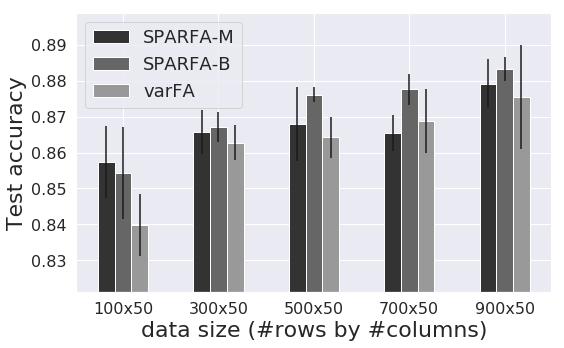
\includegraphics[width=0.4\linewidth]{sim_acc.png}
    \hspace{3pt}
    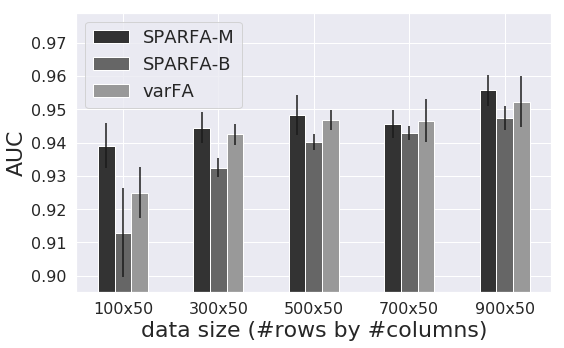
\includegraphics[width=0.4\linewidth]{sim_auc.png}
    \hspace{3pt}
    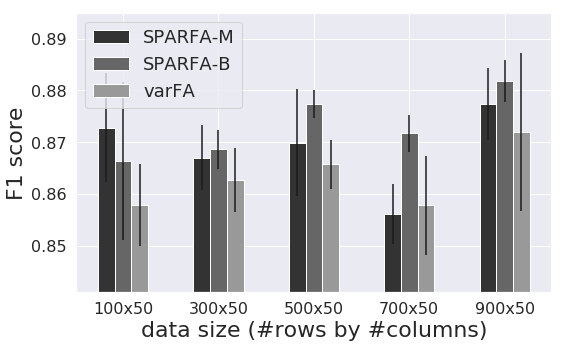
\includegraphics[width=0.4\linewidth]{sim_f1.png}
    \caption{Performance of the  SPARFA-M, SPARFA-B, and VarFA algorithms on the synthetic data set with different data sizes. Plots from left to right show comparison on accuracy (ACC), area under curve (AUC) and F1 metrics, respectively. Higher is better for all metrics. VarFA  performs
        similarly to SPARFA-M and SPARFA-B.}
    \label{fig:synthetic}
\end{figure*}

\subsection{Remarks}
%
\subsubsection*{Applicability of VarFA} The VarFA framework is general and flexible and can be applied to a wide array
of FA models. The recipe for applying VarFA to an FA model of choice is as
follows: 1) formulate the FA model into the canonical formulation as in
Eq.~\ref{eq:sparfa}; 2) partition the factors into student factor $\nu$, the
remaining unknown factors $\theta$ and known factors $\psi$; 3) perform VI on
$\nu$ and MLE estimation on $\theta$, following
Section.~\ref{sec:method-details}.

\subsubsection*{Relation to variational auto-encoders}Our proposed framework can be regarded as a standard variational auto-encoder
(VAE) but with the decoder implemented not as a neural network but by the FA
model. Because the decoder is constraint to a FA model, it is more
interpretable than a neural network.

\subsubsection*{Relation to other efficient Bayesian factor analysis methods}
We acknowledge that VI applied to general FA models have been proposed in
existing literature~\cite{ghahramani2000variational,zhao2009note}. However, to
our knowledge, little prior work have applied VI to educational FA models nor
investigated its effectiveness. One concurrent work applied VI to
IRT~\cite{wu2020variational}. Our VarFA framework applies generally to a number
of other FA models by following the recipe in the preceding paragraph,
including IRT. Thus, our work complements existing literature in providing
promising results in applying VI for FA models in the context of educational
data mining.
%
\section{Experiments}
\label{sec:experiments}
%
We demonstrate the efficacy of VarFA variational inference framework using the
sparse factor analysis model (SPARFA) as the underlying FA model.
%
This choice of SPARFA as the FA model to investigate is motivated by its
mathematical generality: it assumes no auxiliary information is available and
all three factors $\rvc_i$'s, $\rvm_j$'s and $\mu_j$'s need to be estimated,
which makes the inference problem more challenging.~\cite{lan14a} provides two
inference algorithms including SPARFA-M (based on MLE) and SPARFA-B (based on
MAP).
%
We conduct experiments on both synthetic and real data sets. Using synthetic
data sets, we compare VarFA to both SPARFA-M and SPARFA-B. We demonstrate that
1) VarFA predicts students' answers as accurately as SPARFA-M and SPARFA-B; 2)
VarFA is almost 100$\times$ faster than SPARFA-B. Using real data sets, we
compare VarFA to SPARFA-M. We demonstrate that 1) VarFA predicts students'
answers more accurately than SPARFA-M; 2) VarFA can output the same insights as
SPARFA-M, including point estimate of students' skill levels and questions'
associations with skill tags;
% \ml{you can be more specific here about what type of insights do we obtain} 
3) VarFA can additionally output meaningful uncertainty quantification for student skill levels, which SPARFA-M is incapable of, without sacrifice to computational efficiency. Note that SPARFA-B can also compute uncertainty for small data sets but fails for large data sets due to scalability issues and thus we do not compare to SPARFA-B for real data sets.
%
Specifically for SPARFA, using the notation convention in
Section~\ref{sec:FA-inference}, the question-skill association factors
$\rvm_j$'s and the question difficulty factors $\mu_j$ are collected in $\theta
    = \{\rvm_1,...,\rvm_Q,\mu_1,...,\mu_Q\}$. The student skill level factors
$\rvc_j$'s are collected in $\nu = \{\rvc_1,...,\rvc_N\}$. Because the factors
$\rvm_j$'s are unknown, the ``skills'' in SPARFA are \textit{latent} (referred
to as ``latent skills'' in subsequent discussions) and are not attached to any
specific interpretation. However, as we will see in
Section~\ref{sec:experiment-post-processing}, assuming the skill tags are
available as auxiliary information, we can associate the estimated latent
skills with the provided skills tags using the same approach proposed
in~\cite{lan14a}. For the regularization term in Eq.~\ref{eq:objective},
because the factors $\rvm_j$'s are assumed to be sparse and nonnegative, we use
$\ell1$ regularization for $\rvm_j$'s. When performing MLE for $\rvm_j$'s, we
use the proximal gradient algorithm for optimization problem with nonnegative
and sparsity requirements; see Section 3.2 in~\cite{lan14a} for more details.
For the other unknown factor $\mu_j$'s in $\theta$, we apply standard $\ell2$
regularization. The code along with instructions to reproduce our experiments
can be downloaded from~{\color{blue}{\url{https://tinyurl.com/tvm4332}}}.
%
\begin{figure}
    \tiny
    \centering
    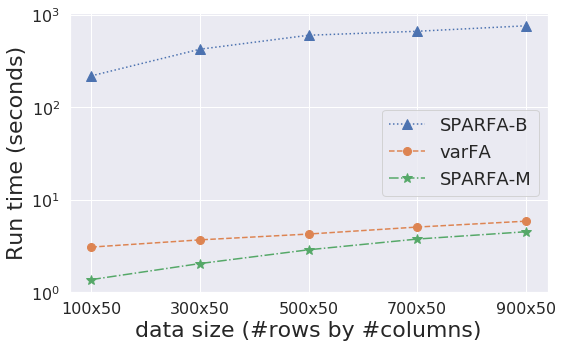
\includegraphics[width=0.4\linewidth]{sim_time.png}
    \caption{Training run time comparing VarFA, SPARFA-M, and SPARFA-B on synthetic data sets of varying sizes. VarFA performs approximate Bayesian inference almost 100x faster than SPARFA-B and is close to the run time of SPARFA-M. Thus, VarFA enables practical and scalable Bayesian inference for very large data sets.}
    \label{fig:run-time}
\end{figure}
\subsection{Synthetic Data Experiments}
\subsubsection{Setup}
%
\subsubsection*{Data set generation} We generate data set according to the canonical FA model specified in
Eq.~\ref{eq:sparfa}, taking into consideration the additional sparsity and
nonnegativity assumptions in SPARFA. Specifically, We sample the factors
$\mu_j$'s and $\rvc_i$'s from i.i.d. standard isotropic Gaussian distributions
with variance $1$ (or identity matrix for $\rvc_i$'s) and mean sampled from a
uniform distribution in range $[-1, 1]$. To simulate sparse and nonnegative
factors $\rvm_j$'s, we first sample an auxiliary variable $s_{kj}\stackrel{\rm
        i.i.d.}{\sim}{\rm Bernoulli}(\pi)$, where $\pi$ controls the sparsity, and then
sample $m_{kj}\stackrel{\rm i.i.d.}{\sim}{\rm Exponential}(1)$ when $s_{kj}=1$
or setting $m_{kj}=0$ when $s_{kj}=0$ for each $j$ and $k$. In all synthetic
data experiments, we use $\pi=0.3$ and set the true number of latent skills to
$K=5$.

%\vspace{-10pt}
\subsubsection*{Experimental settings}
We vary the size of the data set and use 5 different data matrix sizes:
100$\times$50, 300$\times$50, 500$\times$50, 700$\times$50 and 900$\times$50.
We select a data missing rate of 50\%, i.e., we randomly choose 50\% of all
entries in the data matrix as training set and the rest as test set.
Experimental results for each of the above data sizes are averaged over 5 runs
where we randomize over the train/test data split. We train SPARFA with both
SPARFA-M and VarFA using the Adam optimizer~\cite{kingma2014adam} with learning
rate $=0.05$ for 100 epochs. Regularization hyper-parameters are chosen by grid
search for each experiment. For VarFA, we use a simple 3-layer neural network
for the function $f_\phi$ in the variational distribution. We use the
hyper-parameter settings for SPARFA-B following Section 4.2 in~\cite{lan14a}.
%
\begin{table}
    \caption{Summary statistics of pre-processed real data sets.}
    %\vspace{-5pt}
    \begin{tabular}{lccc}
        \toprule
        \textbf{data set}          & \textbf{\#students} & \textbf{\#questions} & \textbf{\%observed} \\ \hline
        assistment \Tstrut \Bstrut & 392                 & 747                  & 12.93\%             \\
        algebra                    & 697                 & 782                  & 13.02\%             \\
        bridge                     & 913                 & 1242                 & 11.42\%             \\ \bottomrule
    \end{tabular}
    \label{tab:data-stat}
\end{table}

%\vspace{-10pt}
\subsubsection*{Evaluation metrics} We evaluate the inference algorithms on their ability to recover (predict) the
missing entries in the data matrix given the observed entries. We term this
criterion ``student answer prediction''. Since our data matrix is binary, using
prediction accuracy (ACC) alone does not accurately reflect the performance of
the inference algorithms under comparison. Thus, we use area under the receiver
operating characteristic curve (AUC) and F1 score in addition to ACC, as
standard in evaluating binary predictions~\cite{hastie2009elements}.
%
\subsubsection{Results}
Fig.~\ref{fig:synthetic} shows bar plots that compare the
%
student answer prediction performance of VarFA with SPARFA-M and SPARFA-B on
all three evaluation metrics. We can observe that all three methods perform
similarly and that SPARFA-M and SPARFA-B show no statistically significant
advantage over VarFA.
\sloppy
We further showcase VarFA's scalability by comparing its training run-time with SPARFA-M and SPARFA-B. The results are shown in Fig.~\ref{fig:run-time}. VarFA is significantly faster than SPARFA-B and is almost as fast as SPARFA-M.

In summary, with VarFA, we obtain posteriors that allow uncertainty
quantification with roughly the \textit{same} computation complexity of
computing point estimates and \textit{without} compromising prediction
performance.
\begin{table}[t!]
    \caption{Student answer prediction erformance comapring VarFA to SPARFA-M on Assistment, Algebra and Bridge data sets. $\uparrow$ and $\downarrow$ denote higher and lower is better, respectively. VarFA performs better than SPARFA-M on all three data sets and evaluation metrics most of the time. Additionally, VarFA's run time is very close to SPARFA-M.}
    % %\vspace{5pt}
    \centering
    \begin{subtable}{\linewidth}\centering
        \caption{Assistment}
        %\vspace{-5pt}
        \begin{tabular}{lcc}
            \toprule
            \textbf{Metric}                            & \multicolumn{2}{c}{\textbf{Algorithm}}                              \\  \hline \\[-8pt]
            % \cmidrule(l){2-2} \cmidrule(l){3-3}
                                                       & SPARFA-M                               & VarFA                      \\
            \cmidrule(l){2-2} \cmidrule(l){3-3}
            ACC $\uparrow$                             & 0.7074$\pm$0.0044                      & \textbf{0.7101}$\pm$0.0048 \\
            AUC $\uparrow$                             & 0.756$\pm$0.048                        & \textbf{0.7635}$\pm$0.0036 \\
            F1 $\uparrow$                              & 0.7746$\pm$0.0029                      & \textbf{0.7765}$\pm$0.0014 \\ \hline
            Run time (s) $\downarrow$  \Tstrut \Bstrut & \textbf{5.3319}$\pm0.2774$             & 6.9167$\pm$0.1074          \\
            \bottomrule
            %\vspace{1pt}
        \end{tabular}
        \label{tab:assistiemnt}
    \end{subtable}
    \begin{subtable}{\linewidth}\centering
        \caption{Algebra}
        %\vspace{-5pt}
        \begin{tabular}{lcc}
            \toprule
            \textbf{Metric}                           & \multicolumn{2}{c}{\textbf{Algorithm}}                              \\  \hline \\[-8pt]
            % \cmidrule(l){2-2} \cmidrule(l){3-3}
                                                      & SPARFA-M                               & VarFA                      \\
            \cmidrule(l){2-2} \cmidrule(l){3-3}
            ACC $\uparrow$                            & 0.7735$\pm$0.0037                      & \textbf{0.7774}$\pm$0.0031 \\
            AUC $\uparrow$                            & 0.8137$\pm$0.003                       & \textbf{0.8245}$\pm$0.002  \\
            F1 $\uparrow$                             & 0.8465$\pm$0.0021                      & \textbf{0.8486}$\pm$0.001  \\\hline
            Run time (s) $\downarrow$ \Tstrut \Bstrut & \textbf{8.464}$\pm$0.4568              & 10.3335$\pm$0.4435         \\
            \bottomrule
            %\vspace{1pt}
        \end{tabular}
        \label{tab:algebra}
    \end{subtable}
    \begin{subtable}{\linewidth}\centering
        \caption{Bridge}
        %\vspace{-5pt}
        \begin{tabular}{lcc}
            \toprule
            \textbf{Metric}                            & \multicolumn{2}{c}{\textbf{Algorithm}}                              \\  \hline \\[-8pt]
            % \cmidrule(l){2-2} \cmidrule(l){3-3}
                                                       & SPARFA-M                               & VarFA                      \\
            \cmidrule(l){2-2} \cmidrule(l){3-3}
            ACC $\uparrow$                             & \textbf{0.8492}$\pm$0.0016             & 0.8468$\pm$0.0016          \\
            AUC $\uparrow$                             & 0.837$\pm$0.0024                       & \textbf{0.8419}$\pm$0.0028 \\
            F1 $\uparrow$                              & \textbf{0.9121}$\pm$0.0005             & 0.912$\pm$0.0009           \\\hline
            Run time (s) $\downarrow$  \Tstrut \Bstrut & \textbf{15.6048}$\pm$0.7314            & 15.8558$\pm$1.046          \\
            \bottomrule
        \end{tabular}
        \label{tab:bridge}
    \end{subtable}
    \label{tab:real-data}
\end{table}

\begin{figure*}[t!]
    \centering
    \begin{subfigure}[b]{0.31\textwidth}
        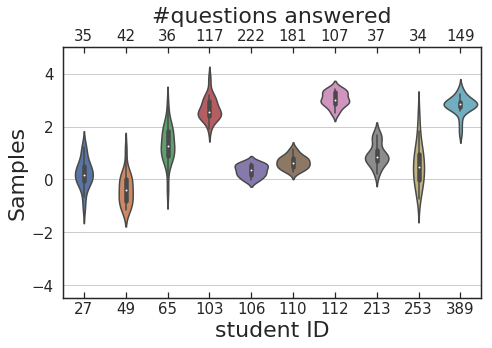
\includegraphics[width=\linewidth]{violin3.png}
        \caption{3rd latent concept}
        \label{fig:violin1}
    \end{subfigure}
    \hspace{5pt}
    \begin{subfigure}[b]{0.31\textwidth}
        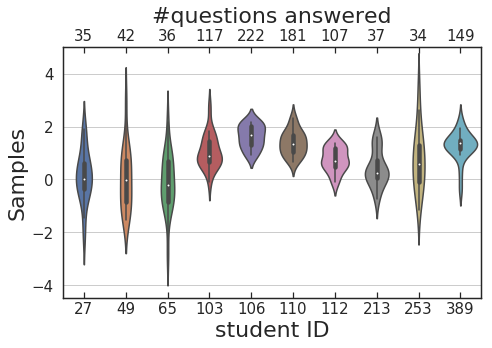
\includegraphics[width=\linewidth]{violin4.png}
        \caption{4th latent concept}
        \label{fig:violin2}
    \end{subfigure}
    \hspace{5pt}
    \begin{subfigure}[b]{0.31\textwidth}
        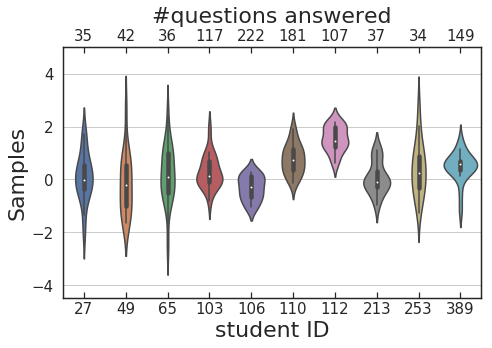
\includegraphics[width=\linewidth]{violin7.png}
        \caption{7th latent concept}
        \label{fig:violin3}
    \end{subfigure}
    \caption{Violin plot showing the mean and standard deviation of the estimated skill mastery levels on 10 selected students on the 3rd, 4th and 7th latent skills that VarFA computes. In each sub-figure, bottom and top axises respectively shows student IDs and top axis shows the number of questions each student answered. The more questions a student answers, the tighter the credible interval. (Best viewed in color.)}
    % \end{subfigure}
    \label{fig:violin}
\end{figure*}

\subsection{Real Data Experiments}
\subsubsection{Setup}
%\vspace{-10pt}
\subsubsection*{Data sets and pre-processing steps} We perform experiments on three large-scale, publicly available, real
educational data sets including ASSISTments 2009-2010 (Assistment)~\cite{assistment}, Algebra I 2006-2007 (algebra)~\cite{Algebra} and Bridge to Algebra 2006-2007 (bridge)~\cite{bridge,Stamper2016The2K}. The details of the data sets, including data format and data collection procedure can be found in the preceding references. We remove students and questions that have too few answer records from the data sets to reduce the sparsity of the data sets. Specifically, we keep students and questions that have no less than 30, 35 and 40 answer records for Assistment, Algebra and Bridge data sets, respectively.
In each data set, each student may provide more than one answer record for each question. Therefore, we also remove student-question answer records except for the first one.
Table~\ref{tab:data-stat} presents the summary statistics of the resulting pre-processed data matrix for each data set.

\subsubsection*{Experimental settings and evaluation metrics} Optimizer, learning rate, number of epochs, neural network architecture and
evaluation metrics are the same as in synthetic data experiments. For real data
sets, we use 8 latent skills instead of 5. Other choices of the number of
latent skills might result in better performance. However, since we are
comparing different inference algorithms for the \textit{same} model, it is a
fair to compare the inference algorithms on the same model with the same number
of latent dimensions.
% \ml{it's better to add an argument here justifying this choice}\jack{attempted a fix}. 
We use a 80:20 data split, i.e., we randomly sample 80\% and 20\% of the
observed entries in each data set, without replacement, as training and test
sets, respectively. Regularization hyper-parameters are selected by grid search
and are different for each data set. We only compare VarFA with SPARFA-M
because SPARFA-B does not scale to such large data sets.
%
\subsubsection{Results: Performance Comparison}
Table~\ref{tab:real-data} shows the average performance on the test set of each
data set comparing VarFA and SPARFA-M for all three data sets and additionally
run time. We can see that VarFA achieves slightly better student answer
prediction on most data sets and on most metrics.
%
Interestingly, recall that, in the preceding synthetic data set experiment,
SPARFA-M performed better than VarFA most of the time. A possible explanation
is that, for synthetic data sets, the underlying data generation process
matches the SPARFA model, whereas for real data sets, the underlying data
generation process is unknown. VarFA's better performance than SPARFA-M for
real data sets implies that VarFA is more robust to the unknown underlying data
generation process. As a result, VarFA may be more applicable than SPARFA-M in
real-world situations.

Table~\ref{tab:real-data} also shows the run time comparison between VarFA and
SPARFA-M; see the last row in each sub-table. We see that both inference
algorithms have very similar run time, showing that VarFA is applicable for
very large data sets. Notably, VarFA achieves this efficiency while also
performing Bayesian inference on the student knowledge level factor.
% 
\subsubsection{Results: Bayesian Inference With VarFA}
We now illustrate VarFA's capability of outputting credible intervals using the
Assistment data set.
%
Fig.~\ref{fig:violin} presents violin plots that show the sampled student
latent skill levels for a random subset of 10 students.
Plots~\ref{fig:violin1},~\ref{fig:violin2} and~\ref{fig:violin3} shows the
inferred students ability for the 3rd, 4th and 7th latent skill dimension. In
each plot, the bottom axis shows the student ID and the top axis shows the
total number of questions answered by the corresponding student. For each
student, the horizontal width of the violin represents the density of the
samples; the skinnier the violin, the more widespread the samples are, implying
the model's less certainty on its estimations.

\begin{table*}[t!]
    \fontsize{8pt}{8pt}\selectfont
    \caption{Illustration of the estimated latent skills with the their top 3 most strongly associated skill tags in the Assistment data set. The percentage in the parenthesis shows the association probability (summed to 1 for each latent skill). We see that the tagged skills associated with each estimated latent skill form intuitive and interpretable groups.
        % \ml{either here in the caption or in the text body, explain what these percentages mean. anything here sums to 1?}\jack{f}
    }
    \centering
    \setlength\heavyrulewidth{0.25ex}
    \begin{tabular}{p{0.45\textwidth}p{0.45\textwidth}}
        \toprule
        \textbf{Latent Skill 1}                                                                                                                                  & \textbf{Latent Skill 3}                                                                                                                                                                             \\ \hline \\[-5pt]
        \begin{tabular}[c]{@{}l@{}}Division Fractions (29.1\%)\\ Least Common Multiple (18.1\%)\\ Write Linear Equation from Ordered Pairs (17.8\%)\end{tabular} & \begin{tabular}[c]{@{}l@{}}Conversion of Fraction Decimals Percents (7.3\%)\\ Addition and Subtraction Positive Decimals (6.8\%)\\ Probability of a Single Event (5.7\%)\end{tabular} \vspace{10pt} \\ \toprule \\[-10pt]
        \textbf{Latent Skill 4}                                                                                                                                  & \textbf{Latent Skill 7}
        % \ml{- measuring CJ's ribs}}                                                                                                  
        \\ \hline \\[-5pt]
        \begin{tabular}[c]{@{}l@{}}Pattern Finding (17.4\%)\\ Histogram as Table or Graph (11.3\%)\\ Percent Of (10.5\%)\end{tabular}                            & \begin{tabular}[c]{@{}l@{}}Volume Sphere (13.4\%)\\ Volume Cylinder (10.4\%)\\  Surface Area Rectangular Prism (10.2\%)\end{tabular}                                                                \\ \bottomrule
    \end{tabular}
\end{table*}

Results in Fig.~\ref{fig:violin} confirms our intuition that the more questions
a student answers, the more certain the model is about its estimation. For
example, students with ID 106, 110 and 389 answered 222, 181 and 149 questions,
respectively, and the credible intervals of their ability estimation is quite
small. In contrast, students with ID 27, 49 and 65 answered far less questions
and the credible intervals of their ability estimation is quite large. This
result implies that VarFA outputs sensible and interpretable credible
intervals. As mentioned in Section~\ref{sec:intro}, such uncertainty
quantification may benefit a number of educational applications such as
improving adaptive testing algorithms.
%
Note that VarFA is able to compute such credible interval as fast as SPARFA-M,
making VarFA potentially useful for even real-time educational systems. In
contrast, SPARFA-M is not capable of computing credible intervals. Although we
may still obtain confidence interval as uncertainty quantification with
SPARFA-M via bootstrapping, i.e., train with SPARFA-M multiple times with
random subsets of the data set and then use the point estimates from different
random runs to compute confidence intervals. However, this method suffers from
two immediate drawbacks: 1) it is slow because we need to run the model
multiple times and 2) different runs result in permutation in the estimated
factors and thus the averaged estimations loss meaning. Given that VarFA is as
efficient as SPARFA-M and the previous drawbacks of SPARFA-M, we recommend
VarFA over bootstrapping with SPARFA-M for quantifying model's uncertainty in
practice.

\subsubsection{Results: Post-Processing for Improved Interpretability}
\label{sec:experiment-post-processing}
SPARFA assumes that each student factor $\nu_i$ identifies a multi-dimensional skill level on a number of ``latent'' skills (recall that we use 8 latent skills in our experiments). As mentioned earlier, these latent skills are not interpretable without the aid of additional information. To improve interpretability,~\cite{lan14a} proposed that, when the skill tags for each question is available in the data set, we can associate each latent skill with skill tags via a simple matrix factorization. Then, we can compute each students' mastery levels on the actual skill tags. We refer readers to Sections 5.1 and 5.2 in~\cite{lan14a} for more technical details.

Although the above method to improve interpretability has already been
proposed,~\cite{lan14a} only presented results on private data sets, whereas
here we presents results on publicly available data set with code, making our
results more transparent and reproducible.

We again use the Assistment data set for illustration. We compute the
association of skill tags in the data set with each of the latent skills and
show 4 of the latent skills with their top 3 most strongly associated skill
tags. We can see that each latent skill roughly identify the same group of
skill tags. For example, latent skill 4 clusters skill tags on statistics and
probability while latent skill 7 clusters skill tags on
geometry. Thus, by simple post-processing, we obtain an interpretation of the
latent skills by associating them with known skill tags in the data.

We can similarly obtain VarFA's estimations of the students' mastery levels on
each skill tags through the above process. In Fig.~\ref{fig:skill}, we compare
the predicted mastery level for each skill tag (only for the questions this
student answered) with the percent of correct answers for that skill tag.
Blue curve shows the empirical student's mastery level on a skill tag by
computing the percentage of correctly answered questions belonging to a
particular skill tag. Orange curve shows VarFA's estimated student mastery
level on a skill tag, normalized to range $[0,1]$.
%
We can see that, when the student gave more correct answers to questions of a
particular skill tag, such as skill tag ID 2, 10, 14 and 30, VarFA also
predicts a higher ability score for these skill tags. When the student gave
more incorrect answers to questions of a particular skill tag, such as skill
tag ID 0, 4 and 27, VarFA also predicts a lower ability score for those skill
tags. Although the correspondence is not perfect, VarFA's predicted student's
mastery levels match our intuition about student's abilities (using the
observed correct answer ratio as an empirical estimate) reasonably well. Thus,
by post-processing, we can interpret VarFA's estimated students' latent skill
mastery levels using the easily understandable skill tags.
\section{Conclusions and Future Work}
\label{sec:conclusion}
We have presented VarFA, a variational inference factor analysis framework to perform efficient Bayesian inference for learning analytics. VarFA is general and can be applied to a wide array of FA models. We have demonstrated the effectiveness of our VarFA using the sparse factor analysis (SPARFA) model as a case study. We have shown that VarFA can very efficiently output interpretable, educationally meaningful information, in particular credible intervals, much faster than classic Bayesian inference methods. Thus, VarFA has potential application in many educational data mining scenarios where efficient credible interval computation is desired, i.e., in adaptive testing and adaptive learning systems. We have also provided open-source code to reproduce our results and facilitate further research efforts.

We outline three possible future research directions and extensions. First,
VarFA currently performs Bayesian inference on the student skill mastery level
factor. We are working on extending the framework to perform full Bayesian
inference for all unknown factors. Extensions to some models such as IRT is
straightforward, as studied in~\cite{wu2020variational}, because all factors
can be reasonably assumed to be Gaussian.

However, some other models involve additional modeling assumptions, making it
challenging to design distributions that satisfy these assumptions. For
example, in SPARFA, one of the factors is assumed to be nonnegative and
sparse~\cite{lan14a}. No standard distribution fulfill these requirements. We
are exploring \textit{mixture} distributions, in particular spike and slab
models~\cite{ishwaran2005spike} for Bayesian variable selection, and methods to
combine them with variational inference,
following~\cite{titsias2011spike,enlighten191553}.

Second, other methods exist that accelerate classic Bayesian inference. Recent
works in large-scale Bayesian inference proposed \textit{approximate} MCMC
methods that scale to large data
sets~\cite{zhang2020csgmcmc,ma2015complete,song2017nice}. Some of these methods
apply variational inference to perform the
approximation~\cite{de2001variational,habib2018auxiliary}. We are investigating
extending VarFA to support approximate MCMC methods.

\begin{figure}
    \centering
    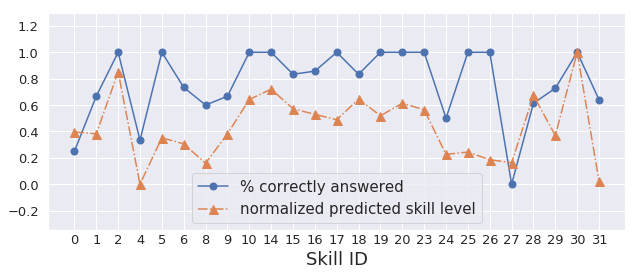
\includegraphics[width=0.8\linewidth]{student_skill.png}
    %\vspace{-15pt}
    \caption{Comparison between the estimated skill mastery levels using VarFA's predictions and using empirical observations for student with ID 110. Even though the two curves show different numeric values, they nevertheless demonstrate similar trends, showing that the predictions reasonably match our intuition about student's skill mastery levels.
        % \ml{caption too long, ugly. move some of this into the text body}
    }
    \label{fig:skill}
    %\vspace{-5pt}
\end{figure}

Finally, the goal of VarFA is to improve real-world educational systems and
ultimately improve learning. Therefore, it is necessary to evaluate VarFA
beyond synthetic and benchmark data sets. We plan to integrate VarFA into an
existing educational system and conduct a case study where students interact
with the system in real-time to understand the VarFA's educational implications
in the wild.
